\documentclass{article}
\usepackage[utf8]{inputenc}
\usepackage{fullpage} % Package to use full page
\usepackage{parskip} % Package to tweak paragraph skipping
\usepackage{amsmath}
\usepackage{hyperref}
\usepackage{cancel}
\usepackage{amssymb}
\usepackage{mathtools}
\usepackage{graphicx} % Required to insert images
\graphicspath{{./figs/}}
\usepackage{varwidth}
\usepackage{amstext}
\usepackage{amssymb}
%\usepackage{float}
\usepackage{array}
\usepackage[dvipsnames]{xcolor}
\usepackage{tikz} % Package for drawing
\usepackage{ctable}
\usepackage{tabu}
\usepackage{longtable}
\usepackage[section]{placeins}
\usepackage{natbib}
\usepackage{multirow}
\usepackage{subfigure}
\usepackage{caption}

\mathtoolsset{showonlyrefs=false}  %Makes it so only referenced equations are labeled 

\setcounter{secnumdepth}{0} %turn off section numbering

\title{The story of the dissipation correction}
\date{}

\newcommand\dsize[1]{\ensuremath{\mathcal{\scriptstyle {#1} } }} % dope new command for dissipation term
\newcommand\ensem[1]{\ensuremath{\left< {#1} \right>}} %ensemble average brakets
\newcommand\fpart[2]{\ensuremath{\frac{\partial {#1}}{\partial {#2} } }} % fractional style partial diff
\newcommand\avg[1]{\ensuremath{ \overline{{#1} }}}
\newcommand{\RN}[1]{%
  \textup{\uppercase\expandafter{\romannumeral#1}}%
}

\makeatletter
\newcommand*\bigcdot{\mathpalette\bigcdot@{.5}}
\newcommand*\bigcdot@[2]{\mathbin{\vcenter{\hbox{\scalebox{#2}{$\m@th#1\bullet$}}}}}
\makeatother

\newenvironment{myeq}   %my totally awesome environment allowing for easy multiline math without too many labels
    {\begin{equation}
    \begin{gathered}
    }
    {
    \end{gathered}
    \end{equation}
    }
\begin{document}

\maketitle

\begin{figure}
    \centering
    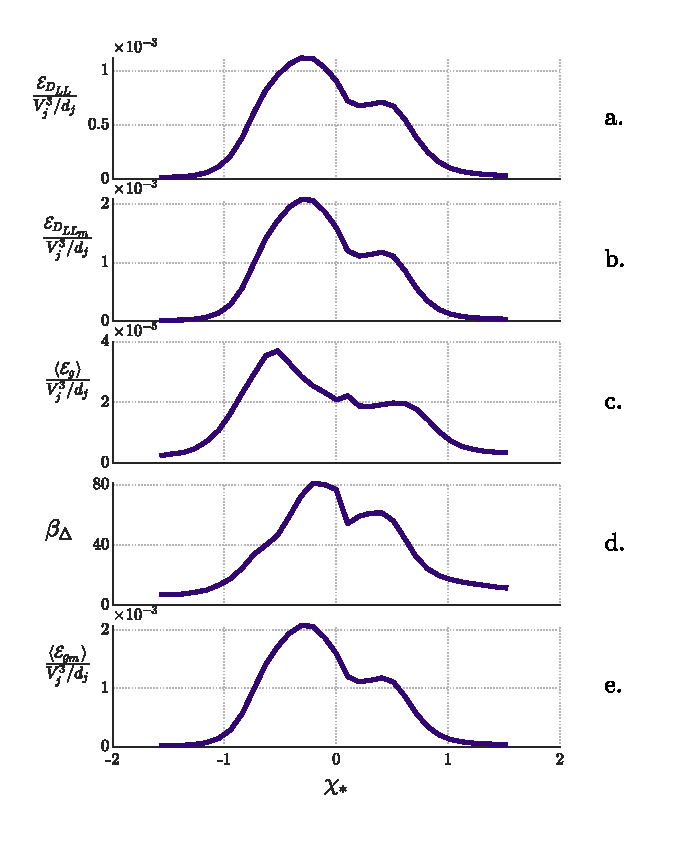
\includegraphics{figs/PG_4Hz_Diss_Splots.eps}
    \caption{Export fig version}
    \label{dissPlots1}
\end{figure}

\begin{figure}
    \centering
    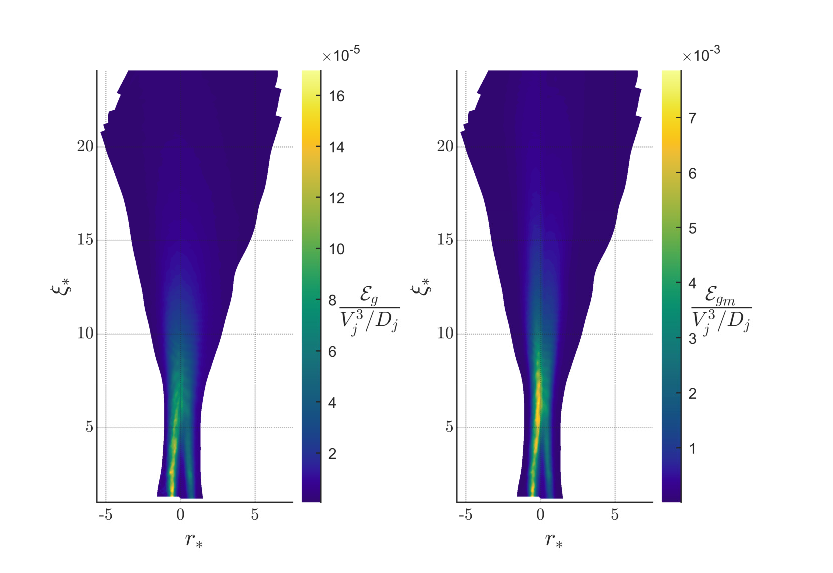
\includegraphics{figs/PG_4Hz_diss_contours.eps}
    \caption{Raw painters}
    \label{conts1}
\end{figure}

\begin{figure}
    \centering
    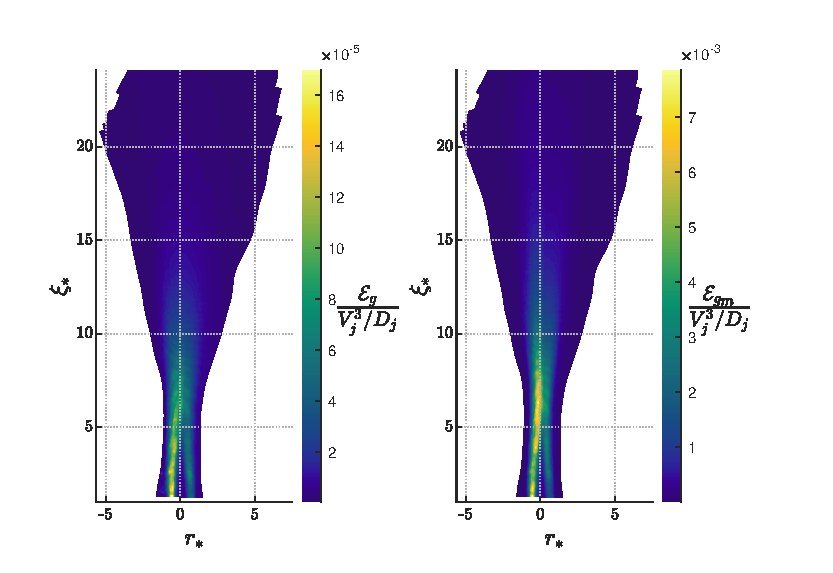
\includegraphics{figs/PG_4Hz_DissConts_CLEAN.eps}
    \caption{Cleaned painters}
    \label{conts2}
\end{figure}

\begin{figure}
    \centering
    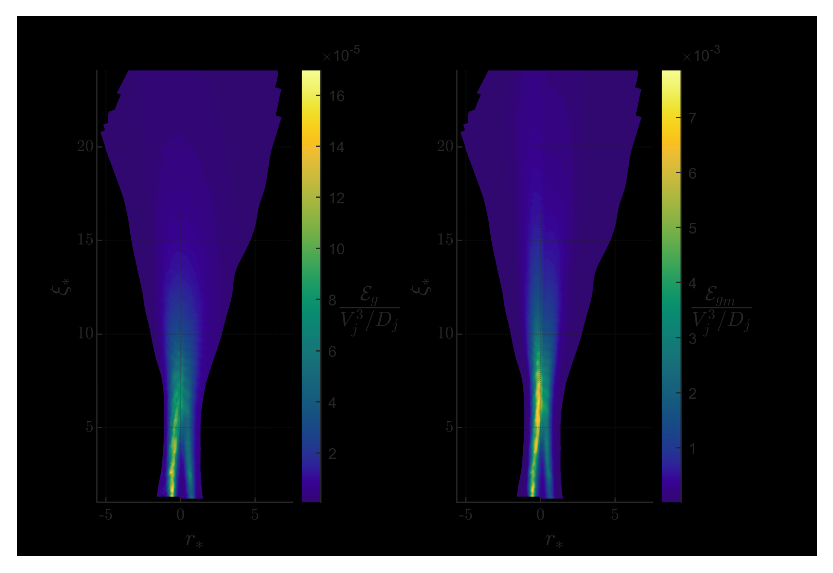
\includegraphics{figs/PG_4Hz_diss_contours2.eps}
    \caption{Raw OpenGl}
    \label{conts3}
\end{figure}

\end{document}
